\section{Introduction}
The taxi rides have been gradually becoming one of the most popular means of public transportation in the major cities all around the world. The path of the taxi rides paint a vivid picture of the life in those cities. It is worth digging into the metadata of the taxi rides to find some useful insight of the city traffic. If we could predict the trip duration of given pickup location, dropoff location during the given time of the day, many stakeholders could potentially benefit from such information. The passengers can determine when is the optimal time to start their commute; the taxi driver can decide which of two potential rides is more profitable; the taxi companies can distribute the cabs more efficiently. 
In this project, we attempted to explore and understand the dataset, 2016 NYC Yellow Cab trip record data, then try to find optimal features and finally the most efficient prediction model. We generated various of features that could potentially affect the final prediction, and then studied the effectiveness and the shortcomes of different models with the given features. In this report, we only talked about three of them: Rigde-regression, neural network, SVR and XGBoosts.   
We evaluated our model based on Root Mean Square Error (RMSE). We used the best model that fits our data and features in our final submission for Kaggle Competition. We use the Kaggle score and the percentile of all submission as an indicator of the quality of our work. The Kaggle scored our model as 0.37734, which ranks 127$th$ (Top 10\%) in the public leaderboard.


\section{Related Work}
With the popularization of the private cars and ridesharing mobile applications like Uber and Lyft, the transportation industry has drawn lots of interests in academic context. Many efforts had been put into the prediction traffic-related information, for instance, the trip duration between two points and the fare of a taxi trip. To predict the trip duration, there are generally two ways: using historical data as training model to predict new data set or using GPS streaming data to perform some near real time prediction. 
In~\cite{antoniades2016fare} authors utilize the same dataset we used in this project, which is Taxi and Limousine Commission’s trip data, to perform series of modeling to predict the trip duration and corresponding fare. They tackled the problem with features that were in original data and the random forest as model to get decent prediction without any real time data. Authors of~\cite{lee2015taxi} also gets similar conclusion that the random forest gives best RMSE among models using different feature extracted from the original dataset. Researchers from IIMA~\cite{laha2017travel} proposed a new model called KNN Regression with Spherical Distance, and perform it on the streaming data, intending to get some real-time insight of the traffic. After comparison with the result they got from some other model such as Support Vector Regression and linear regression, they conclude the KNNRSD worked better when the drop-off location is unknown and the data scale is large. Although GPS streaming data seems more attractive, the blog posts about Google Maps API~\cite{weber_2015} that was released on 2015 shows that the importance of the being able to predict the traffic without real time traffic data.   



\section{Our Approach}

\subsection{Exploratory Data Analysis}
Exploratory data analysis often is considered as the next step to do after people acquire and preprocess data. It is an approach to summarize the main characteristics of the dataset, which help people better understand datasets. With the help of Exploratory Data Analysis, people can possibly choose better models or algorithms to fit data, validate necessary assumptions, and avoid unexpected problems in the following steps.

In our project, we have done EDA to understand the distribution of the given dataset and access necessary assumptions before start modeling. 

Since trip duration was the prediction for our models to make, we were interested in the distribution of all trips provided. We first took the natural logarithm of all trip durations, and then we plotted a histogram as blew. The x-axis is the logarithm of trip duration, and the y-axis is the number of records in training set (Fig.~\ref{fig:eda1}). 

\begin{figure}
	\centering
	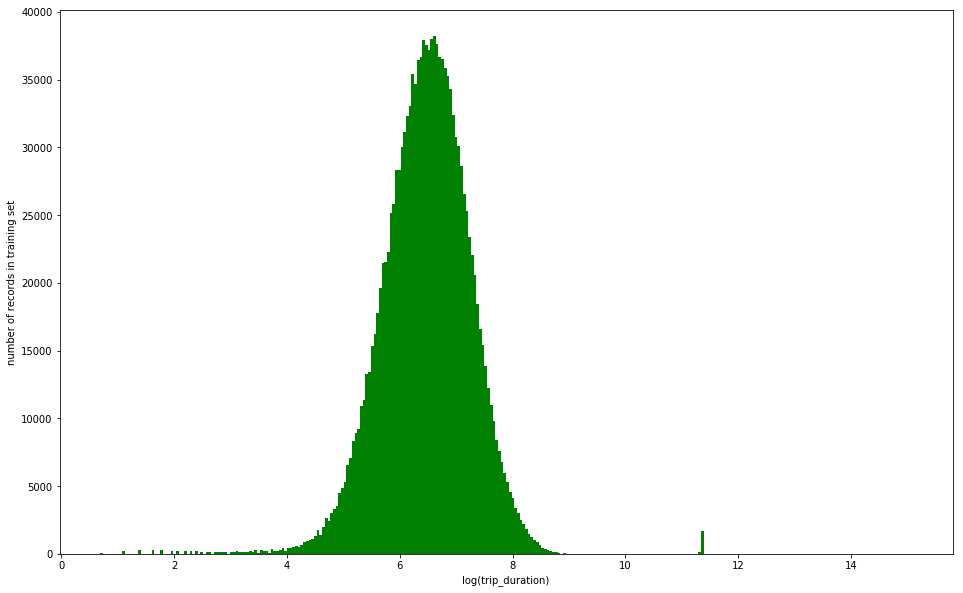
\includegraphics[width=\linewidth]{eda1.png}
	\caption{Taxi Trip Duration Distribution}
	\label{fig:eda1}
\end{figure}

As what we can see from the above histogram, the logarithm of trip durations has a nice gaussian-like distribution except for several some outliers sitting on the right of the main distribution. We went back and checked the maximum value of all trip durations in the training dataset and found the maximum is 979 hours. Apparently, there are some extreme outliers. But fortunately, the evaluation metric for this competition is Root Mean Squared Logarithmic Error, which makes the evaluation much less influenced by outliers. 

Next, we validated whether training set and testing set had the same distribution. This validation was important because most of the machine learning methods would only work well when testing data were drawn from the same distribution. In other words, machine learning could interpolate well, but extrapolation would always be a tough problem. We first checked the pattern of number of records versus date in training set and testing set separately (Fig.~\ref{fig:eda2}). 

\begin{figure*}[!htbp]
	\centering
	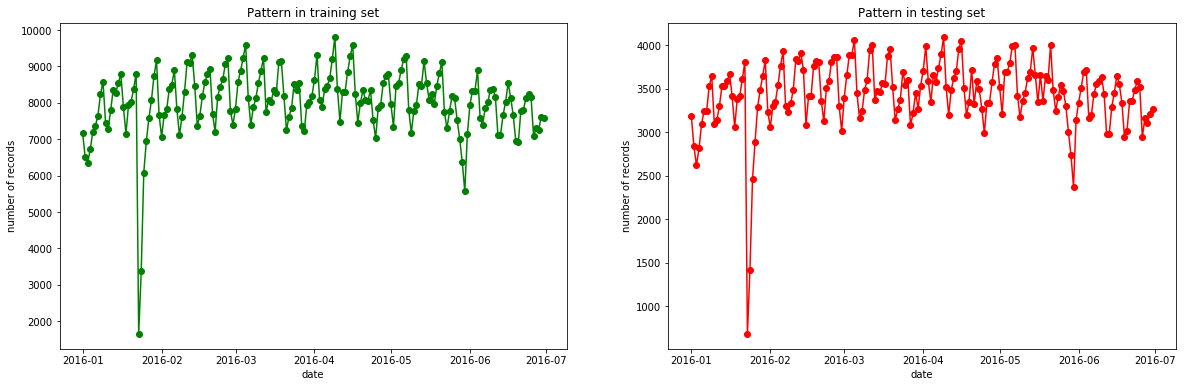
\includegraphics[width=\linewidth]{eda2.png}
	\caption{Number of Trips Across Date in Training (Left) and Testing (Right) Dataset}
	\label{fig:eda2}
\end{figure*}

From the plot above, we could tell that training set and testing set had the same distribution in term of number of records versus date. 

Furthermore, we validated the geometrical distribution of the pickup locations in training and testing sets. As shown as below (Fig.~\ref{fig:eda3}), the pickup locations in training and testing sets overlapped. 

\begin{figure*}[!htbp]
	\centering
	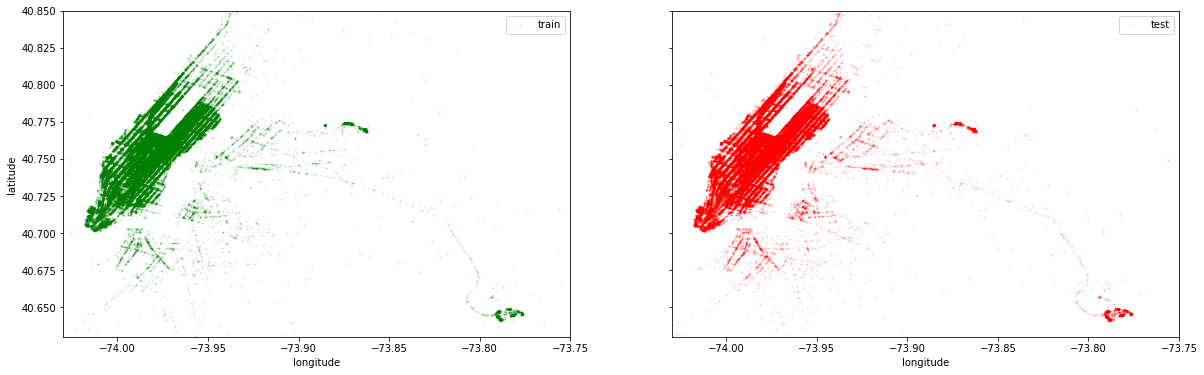
\includegraphics[width=\linewidth]{eda3.png}
	\caption{Pickup Coordinates in Training (Left) and Testing (Right) Dataset}
	\label{fig:eda3}
\end{figure*}

In conclusion, training and testing set overlapped in terms of both temporal and geometrical characteristics, which ensured that we could expect to predict trip durations well by manipulating machine learning techniques. 

\subsection{Feature Engineering}

\subsubsection{PCA Features}
Pickup and dropoff locations are important factors in determining total durations of trips. In the given dataset, geometry locations are represented by longitude and latitude. PCA (Principal Component Analysis) is often used for dimensionality reduction. Here we did 2d to 2d PCA. Although it did not bring benefits by reducing dimensionality, our tree models used later might gain benefits from the rotation done by PCA.

\subsubsection{Distance Features}
Distance is intuitively an important factor for trip duration prediction. To approximately calculate the distance between two given pick-up and drop-off points, we decided to utilize Haversine Formula. The base formula~\cite{wiki:Haversine_formula} is defined as

\begin{equation}
\text{hav}(\theta) = \sin^2(\cfrac{\theta}{2}) = \cfrac{1-\cos(\theta)}{2}
\end{equation}

We use this function to calculate what we called haversine distance. The detailed compute process are as follows: 
\begin{enumerate}
	\item We first use following formula~\cite{wiki:Haversine_formula} to calculate the haversine of the central angle. Note the $\varphi_1, \varphi_2$  are the latitudes of given locations and $\lambda_1, \lambda_2$ are the longitudes of given locations. 
	\begin{equation}
	\text{hav}(\cfrac{d}{r}) = \text{hav}(\varphi_2 - \varphi_1) + \cos(\varphi_1) \cos(\varphi_2) \text{hav}(\lambda_2 - \lambda_1)
	\end{equation}
	\item We denote the haversine of the central angle we got from previous step as h. Then we have~\cite{wiki:Haversine_formula}:
	\begin{equation}
	d = r \text{hav}^{-1}(h) = 2 r \arcsin(\sqrt{h})
	\end{equation}
\end{enumerate}
The haversine distance is good for estimating the great-circle distance between two points on a sphere given their longitudes and latitudes, even the distance is relatively small (some other way of distance calculating is not accurate when distance is small)~\cite{scripts2013calculate}. Because of the good quality of distance estimation, we use haversine distance to calculate average speed denoting as $avg\_speed\_h$ in later steps.  

Manhattan distance (or Taxicab Distance in some context) is another supplementary way of calculating the distance for this distance. The manhattan distance~\cite{wiki:Taxicab_geometry} is defined as sum of the lengths of the projections of the line segment between the points onto the coordinate axes. In the plane case, the Manhattan distance between them equals $|x_1-x_2|+|y_1-y_2|$, where $(x_1, y_1)$, $(x_2, y_2)$ are the coordinates of two points. In our case, the two coordinates would be the longitudes and latitudes pair of the pickup and dropoff locations. Since the points given in our context are on a sphere instead of a plane, we have to perform haversine function on dataset consisted of two points with same latitudes, different longitudes and two points with same longitudes and different latitudes. Then we simply add the absolute values of two haversine results together. The manhattan distance is a more indirect way of determining the distance, but the result will not be so far away from result from haversine formula in practice. We use the $manhattan\_distance$ as a feature to calculate average speed denote as $avg\_speed\_m$. 

Another factor we may want to take into consider is the direction or the bearing of the taxi. Only knowing the distance between two points could not tell the direction of the movement. Here we need to find a way to calculate the direction in terms of the angle of how the heading away from the North. We use the following formula~\cite{scripts2013calculate} to calculate the heading of the taxi: 

\begin{equation}
\theta = \arctan^2(\sin \triangle\lambda \cos \varphi_2, \cos \varphi_1 \sin \varphi_2-\sin \varphi_1 \cos \varphi_2 \cos\triangle \lambda)
\end{equation}

\subsubsection{Datetime Features}
Date and time  which are given in the dataset could also be important factors in determining trip duration. Intuitively, trip duration could be influenced by date because traffic condition varies from date to date. For example, traffic might be heavier during weekdays and smoother during weekend, because some people might tend to go out of town for recreational activities or stay at home. Also, different hours might influence the duration of a trip a lot. Passengers who take trips during peak hours tend to spend more time, and trips that happen at midnight tend to complete in shorter duration. 

Datetime features in raw data are  in the format of “year-month-date hour:minute:second”. We separated it into several features including $pickup\_weekday$, $pickup\_hour\_weekofyear$, $pickup\_hour$, $pickup\_minute$, $pickup\_dt$ and $pickup\_week\_hour$.

\subsubsection{Speed Features}
Here we calculated the average speed for each trip in the dataset. Trip duration and distance were required to derive the average speed. Trip duration could be obtained by comparing the end time and the start time of the trip. For distance, we used two distances derived in 3.2.2, which were Haversine distance and Manhattan distance. We named two newly added speed features $avg\_speed\_h$, $avg\_speed\_m$. 

\subsubsection{Clustering Features}
To explore the possible patterns hidden in the coordinates (i.e., longitude and latitude) for pick-up and drop-off, we employ the classic clustering method, k-means, to the coordinates features, and newly generated cluster labels are used as the new feature.
Considering that the training procedure for k-means might be time-consuming, we adopt an variation of k-means called mini-batch k-means~\cite{sculley2010web}. With the same idea as mini-batch gradient descent, to economize on the computational cost, mini-batch k-means randomly chooses a batch of samples, and then perform the similar steps of vallina k-means to the chosen batch in each iteration until convergence. Experiments \cite{sculley2010web} demonstrate that mini-batch k-means  gets results of slightly lower quality but can largely reduce the convergence time.

\begin{algorithm}
	\caption{Mini-batch $k$-Means}
	\begin{algorithmic}[1]
	\State Givens: $k$, mini-batch size $b$, iterations $t$, dataset $X$ 
	\State Initialize each $c \in C$ with $x$ picked randomly from $X$
	\State $v \gets 0$
	\For{$i=1$ to $t$}
	\State $M \gets b$ examples picked randomly from $X$
	\For{$x \in M$}
	\State $d[x] \gets f(X,x)$
	\EndFor
	\For{$x\in M$}
	\State $c \gets d[x]$
	\State $v[c] \gets v[c] + 1$
	\State $\eta \gets \frac{1}{v[c]}$
	\State $c \gets (1-\eta)c+\eta x$
	\EndFor
	\EndFor
	\end{algorithmic}
\end{algorithm}

\subsubsection{Temporal and Geospatial Aggregation Features}
Due to some regularity of the trips of people in urban area, it is reasonable to analyze the potential patterns after aggregating the temporal or geospatial features. Thus, we conduct the following different aggregation:
\begin{enumerate}
	\item Temporal Aggregation Features:
 We aggregate the speed feature and duration feature by the groupby key-temporal features such as pickup hour, pickup date, etc.
\item Geospatial Aggregation Features:
We aggregate the speed feature and duration feature by the groupby key-coordinates (i.e., latitude and longitude).
\item Clustering Aggregation Features:
Cluster labels can provide implicit patterns associated with each cluster. So, we also count the inflow and outflow of each cluster during a time interval of 60 minutes. Here, we calculate the inflow (outflow) as the number of drop-off (pick-up).
\item Hybrid Aggregation Features:
Temporal and geospatial features are closely tied. For example, the number of pick-up should be large at some office buildings during the rush hour. So, we choose to aggregate the speed feature by multiple group by keys like pick-up hour and coordinates.
\end{enumerate}

\subsubsection{OSRM}
The previous distances are only roughly estimation of the actual distance between points. Given that the cabs are driven on the streets of NYC, we have to determine the path that cabs are actually running on. To achieve this, we use an online open source project called OSRM~\cite{huber2016osrmtime} which can calculate the shortest path in given road networks. Thanks to the pre-populated dataset shared by username oscarleo through Kaggle competition discussion, we could directly use the fastest path from pickup location to dropoff location using OSRM. We extracted several useful features, $total\_distance$, $total\_travel\_time$ from the pre-populated data. The OSRM version of distance and travel time provides more accurate estimation of the path that cabs will really pass by.  	  



\subsection{Data Imputation and Standardization}
We put this step here because there is no missing data in the original dataset. After feature engineering, newly-added features have some missing values. So, data imputation is necessary for the subsequent modeling parts. Note that XGBoost is invariant to the data scale and can deal with missing value well. So, this part is performed for XGBoost.

We employ Multiple Imputation by Chained Equations (MICE)~\cite{azur2011multiple} to conduct data imputation. MICE is one of the principled methods of dealing with missing data. It creates multiple imputation and uses regression models to predict the missing values.

Then, we transform the data by removing the mean and scaling to the unit variance for the purpose of data standardization.
\subsection{Modeling}
\subsubsection{Ridge Regression}
Ridge regression is a linear regression model with L2 regularization. Its objective function is
\begin{equation}
\mathcal{L} = \|y - Aw\|_2^2 + \lambda \|w\|^2_2,
\end{equation}
where $\lambda$ is the shrinkage parameter which controls the amount of regularization. To tune this parameter, we perform the grid search method with cross-validation.

\subsubsection{Neural Network}
We construct a 5-layer Neural Network (Including the output layer). The layer size are 256, 128, 128, 64, 1 respectively. The activation functions are all ReLU. We also employ Batch Normalization to make the input zero-mean and unit-variance. To solve the overfitting problem, we introduce Dropout and Early Stopping strategies. The architecture of the network is shown in Fig.~\ref{fig:nn1}

\begin{figure}[!htbp]
	\centering
	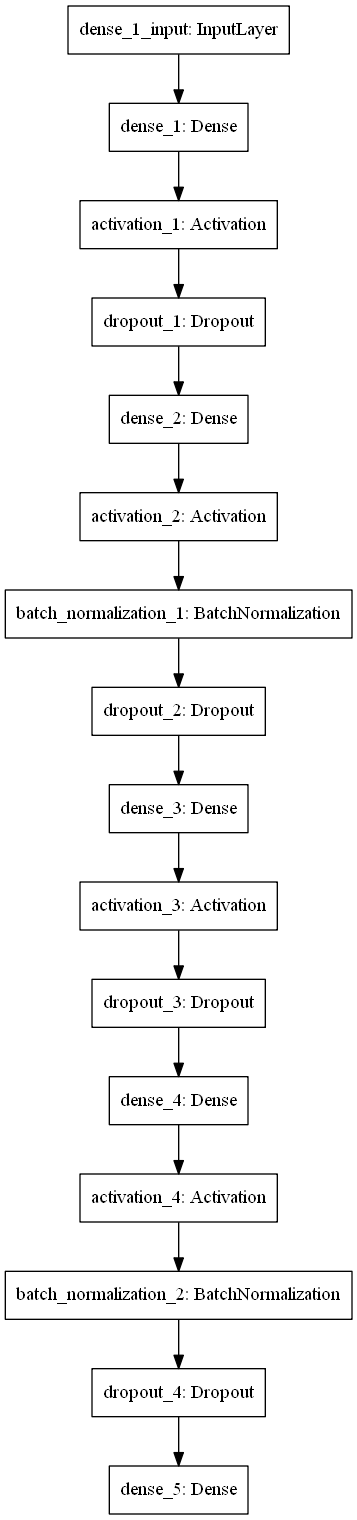
\includegraphics[width=0.55\linewidth]{nn1.png}
	\caption{Architecture of Neural Network}
	\label{fig:nn1}
\end{figure}

\subsubsection{XGBoost}
As one of the most popular methods in the Kaggle Competition and other data mining competitions, eXtreme Gradient Boosting (XGBoost) has been empirically proven to be powerful for machine learning tasks. Its salient strength is the scalability in all the scenarios~\cite{chen2016xgboost}. XGBoost can run several times faster than many other machine learning methods with limited resources. This mainly benefits from the algorithm and system optimization, which is exactly the innovation and novelty in XGBoost. 

Basically, XGBoost is a gradient boosting model (GBM). It builds a strong predictor (classifier) by ensembling the weak ones in a stage-wise manner.

The prediction is calculated as follows.
\begin{equation}
\hat{y}_i = \sum_{k=1}^K f_k(x_i),\ f_k \in \mathcal{F}
\end{equation}
where $f_k$ is the regression tree, $\mathcal{F} = \{f(x) = w_{q(x)}\ (q: \mathbb{R}^m \rightarrow T, w\in \mathbb{R}^T)$, $w$ is an vector which contains the leaf scores, and $q$ represents the tree structure whose output is the leaf index.

To make a good bias-variance trade-off (i.e., generate a predictive and simple model), XGBoost add regularization on the number of leaves and the leaf scores with L2 regularization. Thus, the objective function is
\begin{equation}
\begin{aligned}
& \mathcal{L} = \sum_i l(\hat{y}_i, y_i) + \sum \Omega(f_k) \\
&\text{where } \Omega(f) = \gamma T + \frac{1}{2}\lambda \|w\|^2
\end{aligned}
\label{eq:obj}
\end{equation}

Then, additive training is used to optimize the Eqn.~\eqref{eq:obj}. That is, new function $f_t$ is iteratively added to the prediction function to minimize the objective function in a greedy fashion. Then take the taylor expansion of the objective function
\begin{equation}
\begin{aligned}
\mathcal{L}^{(t)} & = \sum_{i=1}^n l(y_i, \hat{y}_i^{(t-1)}+f_t(x_i)) + \Omega(f_t) \\
&= \sum_{i=1}^n \left( l(y_i, \hat{y}_i^{(t-1)}) + g_if_t(x_i) + \frac{1}{2} h_i f_t^2(x_i)\right) + \Omega(f_t)\\
&= \sum_{j=1} \left((\sum_{i\in I_j} g_i)w_j + \frac{1}{2} (\sum_{i\in I_j h_i + \lambda })w_j^2\right) +\gamma T
\end{aligned}
\end{equation}

Thus, for a fixed tree structure (i.e., $q$), it is easy to acquire the optimal weight for leaf (i.e., $w$).

For the split finding algorithm, instead of the classic method which enumerates all the possible splits and calculate the information gain, XGBoost uses candidates points to get the bucket splits and aggregate them for the purpose of efficiency.
 

\section{Submission and Results}
In this section, we will report and assess the performance of different models used on the NYC taxi dataset. The metric we used for evaluating the four models we attempted on dataset is the Root Mean Square Error (RMSE). 

\begin{equation}
\epsilon = \sqrt{\frac{1}{n}\sum_{i=1}^n(\log(\hat{y}_i + 1) - \log(y_i+1))}
\end{equation}

We also submit our best model to Kaggle from where we can get a LB score. Comparing with other submissions we could know the overall performance of our solution. 

The experiments were carried out on the Amazon Web Service (AWS) platform. The Amazon Machine Image (AMI) is Bitfusion Ubuntu 14 TensorFlow. The instance type is g2.8xlarge with 60 GB RAM and Intel Xeon E5-2670 processor 2.6 GHz with 64 bit Linux 3.13.0.

All the codes are written in Python 3.4.0. The machine learning packages we used include Scikit-Learn and Keras.

The dataset is acquired from Kaggle. The detailed information is listed in Table~\ref{tab:dataset}.

\begin{table}[!htbp]
	\caption{Dataset Information}
	\begin{tabular}{cccc}
		\toprule
		Dataset & Size(MB) & \#Sample & \#Feature \\
		\midrule
		Training & 191& 1,458,644& 10 \\
		Testing & 68 & 625,134& 10\\
		\bottomrule
	\end{tabular}
\label{tab:dataset}
\end{table}

\subsubsection{Ridge Regression}
We use grid search with cross-validation to tune the shrinkage parameter in the space of $[0.001, 0.01, 0.05, 0.1, 0.5, 1, 10]$. The tuning results show that 10 is the best choice with the $RMSE$ of 0.4965 in the validation set.

\subsubsection{Neural Network}
We train the neural network by the Adam Optimizer with the learning rate of $2e-3$ and decay of $1e-3$. The batch size is 32, default for Keras. The epoch is set to 50.

The training results are shown in Fig.~\ref{fig:nn2}

\begin{figure}[!htbp]
	\centering
	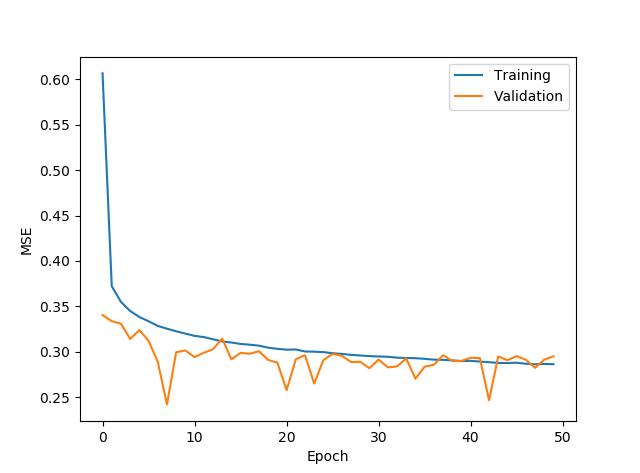
\includegraphics[width=\linewidth]{nn2.png}
	\caption{MSE in Training and Validation Set for NN}
	\label{fig:nn2}
\end{figure}

The training of the Neural Network takes more than 5 hours. Due to the time limitation, we do not have enough time to carefully tune the network.

\subsubsection{XGBoost}
We conducted careful hyperparameter tuning for XGBoost by Grid Search, since the training of XGBoost is quite fast.

The best parameter setting are listed in Table~\ref{tab:xgboost}

\begin{table}[!htbp]
	\caption{XGBoost Hyperparameters}
	\label{tab:xgboost}
	\begin{tabular}{cc}
		\toprule
		Hyperparameter & Value \\
		\midrule
		$min\_child\_weight$ & 10\\
		$eta$ & 0.05\\
		$colsample\_bytree$ & 0.3\\
		$max\_depth$ & 10\\
		$subsample$ & 0.8\\
		$lambda$ & 2\\
		$booster$ & gbtree\\
		$silent$ & 1\\
		$eval\_metric$ & rmse\\
		$objective$ & reg:linear\\
		\bottomrule
	\end{tabular}
	\label{tab:dataset}
\end{table}

The training results are shown in Fig.~\ref{fig:xgboost1}

\begin{figure}[!htbbp]
	\centering
	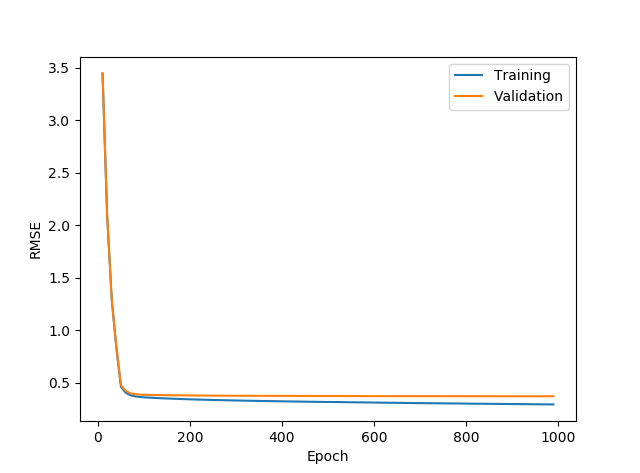
\includegraphics[width=\linewidth]{x1.png}
	\caption{Training Results of XGBoost}
	\label{fig:xgboost1}
\end{figure}

We submitted the results of the best model to Kaggle, and got the score of 0.37734, ranking 127$th$ in the public leaderboard.

\begin{figure}[!htbp]
	\centering
	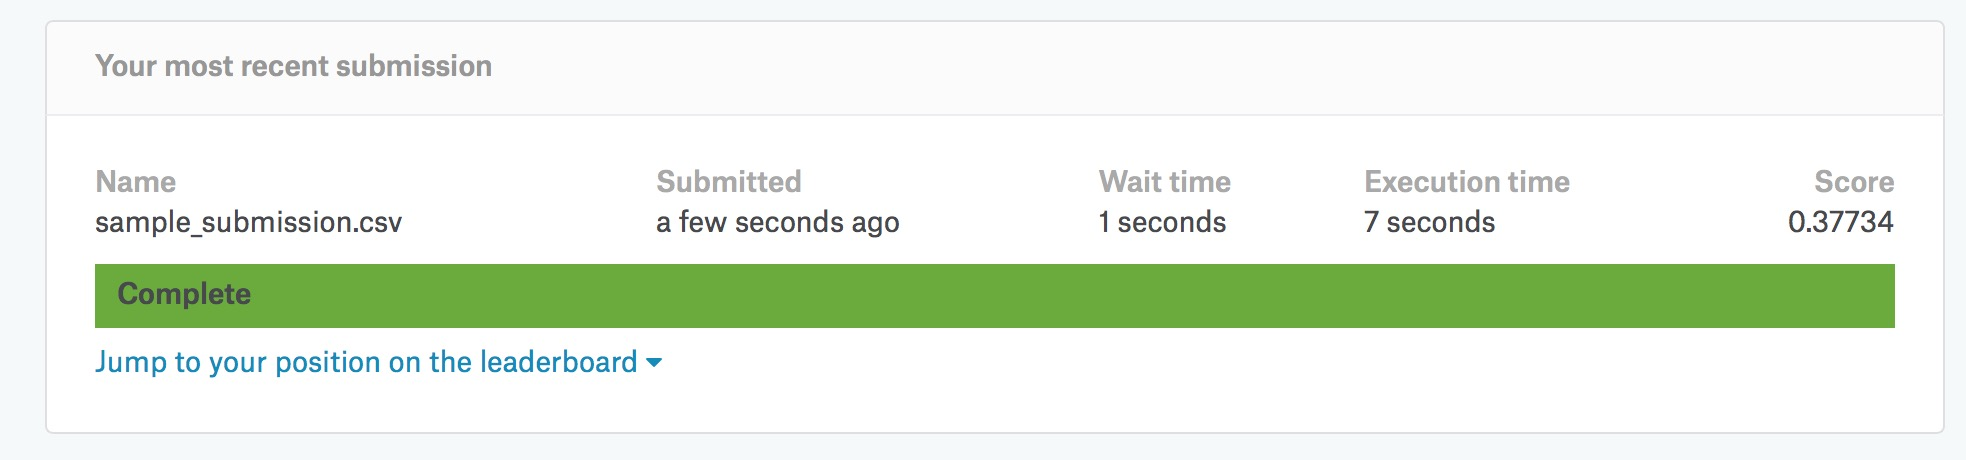
\includegraphics[width=\linewidth]{score.jpg}
	\caption{Score in Kaggle}
\end{figure}

\begin{figure}[!htbp]
	\centering
	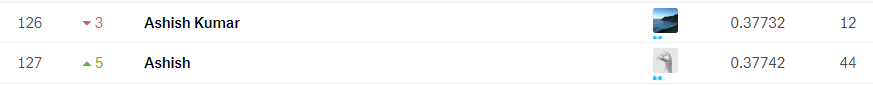
\includegraphics[width=\linewidth]{rank.png}
	\caption{Ranking in Kaggle}
\end{figure}

\section{Conclusion}


\begin{acks}
  The authors would like to sincerely thank Prof. Sahai, Prof. Stellar and TAs in CS289A for meticulous teaching
  and enlightening guidance during this semester.
  
  The authors would also like to thank Beluga and DrGuillermo for their great kernels in Kaggle, which inspire us a lot in the parts of EDA and feature engineering.
  
  The authors would also like to thank Kaggle for providing dataset and hosting such a great competition.

\end{acks}
